\documentclass[
    NAME={Dr. Helga Ingimundardóttir},
    EMAIL={helgaingim@hi.is},
    FACULTY={Industrial Engineering},
    TITLE={Designing Authentic Industry-Engaged Assessment for Professional Competence in Business Intelligence},
    SEMINAR={22\textsuperscript{nd} International CDIO Conference},
    DATE={June 22\textsuperscript{nd} 2026},
    WIDE=true
]{HI-LaTeX/hi-beamer}

\usepackage{tikz}
\usetikzlibrary{fit,matrix,backgrounds}
\usepackage[fixed,style=solid]{fontawesome7}

\begin{document}

%------------------------------------------------

\begin{frame}{Motivation}

\begin{block}{\faBuildingColumns~Academia}
Aims to prepare students for professional practice, but offers limited guidance on how to operationalize this in course design and assessment.
\end{block}

\begin{block}{\faIndustry~Industry}
Expects credible, reproducible results supported by clear reasoning and usable for decision-making.
\end{block}

\begin{alertblock}{Contrasting evaluation perspectives (cause for tension)}
    \begin{itemize}
        \item[\faBuildingColumns] methods and iteration (errors acceptable if reasoning is sound)
        \item[\faIndustry] credibility in context (early errors can undermine trust)
    \end{itemize}        
\end{alertblock}

\end{frame}

%------------------------------------------------

\begin{frame}{Framing the problem}
\begin{exampleblock}{\faDumbbell~Core challenge}
How do we assess \emph{professional competence} in team-based, open-ended projects?    
\end{exampleblock}
\begin{columns}[T]
    \begin{column}{.5\textwidth}
    Particularly:
    \begin{itemize}
        \item collaboration
        \item reasoning and justification
        \item reproducibility
    \end{itemize}    
    \end{column}
    \begin{column}{.5\textwidth}
    Standard assessment:
    \begin{itemize}
        \item often focuses on outputs
        \item weak visibility into process and contribution
    \end{itemize}        
    \end{column}
\end{columns}
\end{frame}

%------------------------------------------------

\begin{frame}{Context: Business Intelligence course}
\begin{columns}[T,onlytextwidth]

\begin{column}{0.38\textwidth}
\begin{exampleblock}{\faMagnifyingGlassChart~Overview}
    \begin{itemize}
        \item 6 ECTS course (advanced undergraduate / early graduate)
        \item 10--15 students, two teams
        \item Semester-long project with \emph{industry partner}
        \item Five modules + Capstone
    \end{itemize}
\end{exampleblock}
\end{column}

\begin{column}{0.58\textwidth}
\begin{block}{\faDatabase~What is BI?}
    Data-driven decision support: combining data analysis, systems, and communication to inform organizational decisions.
\end{block}
\vfill
\begin{block}{\faBullseye~Goal}
    Strengthen industrial relevance and professional competence
\end{block}
\end{column}
\end{columns}



\end{frame}

%------------------------------------------------

\begin{frame}{Design approach}
\begin{columns}[T,onlytextwidth]

\begin{column}{.35\textwidth}
\begin{itemize}
    \item CDIO-aligned redesign
    \item Assessment as \emph{developmental mechanism}
\end{itemize}
\begin{alertblock}{\faKey~Key idea}
\centering
$\begin{array}{cl}
   &  \faComments\ \text{feedback} \\
 + &  \faRepeat\ \text{iteration} \\
 \Rightarrow & \faMedal\ \text{competence}
\end{array}$
\end{alertblock}

\end{column}

\begin{column}{.61\textwidth}

\begin{block}{LOUIS framework}
\small
\textbf{Learning Outcomes in University for Impact on Society}

Focus on a small set of competences (max 3)

\end{block}
\vspace{0.3em}

\centering
\resizebox{\linewidth}{!}{\tikzset{
  compbox/.style={
    draw, rounded corners=5pt, align=center,
    text width=30mm, minimum height=8mm,
    font=\scriptsize, inner sep=1pt
  },
  highlight/.style={
    compbox,
    fill=green!20, draw=green!60!black, very thick
  }
}

\begin{tikzpicture}
  \matrix[matrix of nodes,
          nodes={compbox},
          column sep=2mm, row sep=2mm] {
    {Civic engagement} &
    {Creative thinking} &
    {Critical thinking} &
    {Ethical reasoning} \\
    {Global learning} &
    |[highlight]| {Information literacy} &
    {Inquiry and analysis} &
    {Integrative learning} \\
    {Intercultural knowledge \& competence} &
    {Foundations for life-long learning} &
    {Oral communication} &
    |[highlight]| {Problem solving} \\
    {Quantitative literacy} &
    {Reading} &
    |[highlight]| {Teamwork} &
    {Written communication} \\
  };
\end{tikzpicture}}

\end{column}
\end{columns}
\end{frame}

%------------------------------------------------

\begin{frame}{Pedagogical structure}
\centering\resizebox{.8\linewidth}{!}{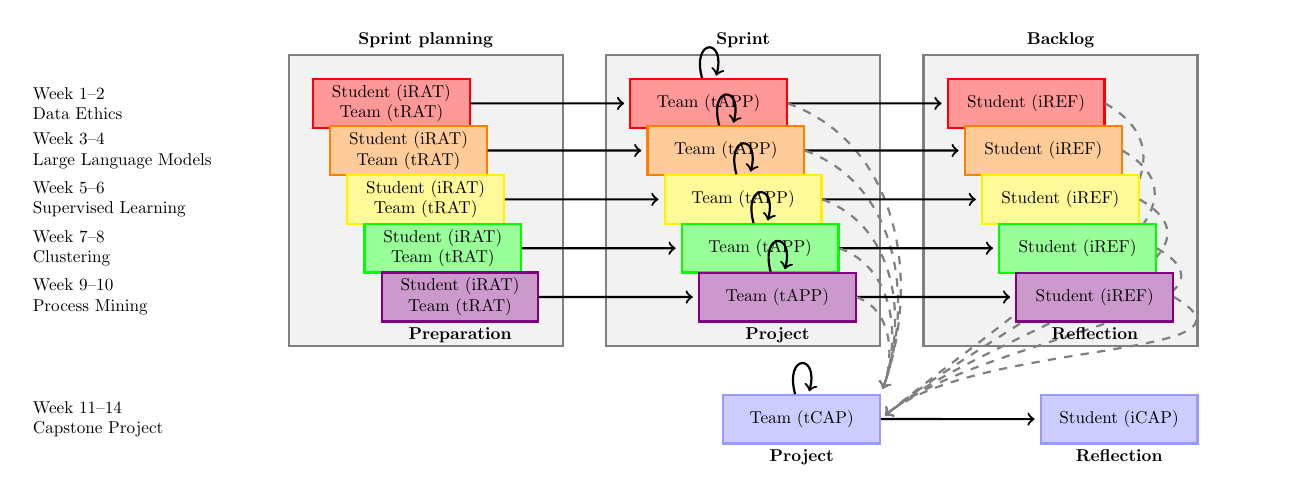
\begin{tikzpicture}
    [scale=0.62, transform shape,
    node distance=65mm,
    inner sep=3pt,
    auto,
    block/.style={
        draw,
        thick,
        fill=green!40,
        text width=30mm,
        align=center,
        minimum height=10mm
    },
    line/.style={
        draw, thick, ->, shorten >=2pt
    },
    dashedline/.style={
        draw, thick, ->, dashed, shorten >=2pt, color=black!50
    },
    week/.style={anchor=south west, text width=45mm},
    red/.style={block, draw=red, fill=red!40},
    orange/.style={block, draw=orange, fill=orange!40},
    yellow/.style={block, draw=yellow, fill=yellow!40},
    green/.style={block, draw=green, fill=green!40},
    violet/.style={block, draw=violet, fill=violet!40},
    blue/.style={block, draw=blue!40, fill=blue!20},
    agile/.style={block, draw=gray, fill=gray!10,inner sep=3mm}
    ]

    % Samantektarverkefni
    \node[week] (themecapstone) at (0,-75mm) {Week 11--14\\ Capstone Project};
    \node[blue, right of=themecapstone, xshift=70mm, label=below:\textbf{Project}] (capstone) {Team (tCAP)};
    % Endurgjöf milli teyma
    \draw [line] (capstone) edge[loop above] (capstone);
    \node[blue, right of=capstone, label=below:\textbf{Reflection}] (capref) {Student (iCAP)};
    \draw[line] (capstone) to (capref);

    % Litur/lotur
    \foreach \week/\theme/\color/\pos in {1--2/Data Ethics/red/1, 3--4 /Large Language Models/orange/2, 5--6/Supervised Learning/yellow/3, 7--8 /Clustering/green/4, 9--10/Process Mining/violet/5}{
        \node[week] (week\pos) at (0,-\pos*10mm) {Week \week\\\theme};
        \node[\color, right of=week\pos, xshift=-50+10*\pos,label=below:\textbf{Preparation}] (RAT\pos)  {Student (iRAT)\\Team (tRAT)};
        \node[\color, right of=RAT\pos,label=below:\textbf{Project}] (APP\pos) {Team (tAPP)};
        \node[\color, right of=APP\pos,label=below:\textbf{Reflection}] (REF\pos) {Student (iREF)};

        % Línur milli eininga
        \path [line] (RAT\pos) -- (APP\pos);
        \path [line] (APP\pos) -- (REF\pos);

        % Jafningjamat innan Teams
        \draw [line] (APP\pos) edge[loop above] (APP\pos);
        
        % Tengingar við samantektarverkefni
        \path [dashedline] (APP\pos.east) to[out=-20, in=70] (capstone.north east);
        \path [dashedline] (REF\pos.east) to[out=-30, in=40] (capstone.east);
    }
    \begin{scope}[on background layer]
    \node[agile,fit=(RAT1) (RAT5),label=above:{\textbf{Sprint planning}}] () {};
    \node[agile,fit=(APP1) (APP5),label=above:{\textbf{Sprint}}] () {};
    \node[agile,fit=(REF1) (REF5),label=above:{\textbf{Backlog}}] () {};
    \end{scope}
\end{tikzpicture}
}
\begin{columns}[T,onlytextwidth]
    \begin{column}{.45\textwidth}
        \begin{itemize}
            \item[\faUserPlus] Team-Based Learning (TBL):
            \begin{itemize}
                \item[\faUser] iRAT (individual readiness)
                \item[\faUsers] tRAT (team readiness)
                \item[\faUsers] tAPP (team application)
                \item[\faUser] iREF (individual reflection)
            \end{itemize}
        \end{itemize}        
    \end{column}
    \begin{column}{.55\textwidth}
        \begin{itemize}            
            \item[\faShuffle] Flipped classroom
            \item[\faRepeat] Iterative modules leading into capstone
        \end{itemize}                
    \end{column}
\end{columns}
\end{frame}

%------------------------------------------------

\begin{frame}{Core mechanism: assessment as development}

\begin{exampleblock}{\faListCheck~One rubric, many iterations}
Same assessment rubric reused across all modules and the capstone

\vspace{.3em}

\small\textit{Standards fixed; performance expectations scaled during learning}
\end{exampleblock}

\begin{columns}[T,onlytextwidth]
\begin{column}{.48\textwidth}
\begin{block}{\faClipboardCheck~Assessment criteria}
\begin{itemize}
    \item analytical soundness
    \item transparency
    \item reproducibility
    \item stakeholder relevance
\end{itemize}
\end{block}
\end{column}

\begin{column}{.48\textwidth}
\begin{alertblock}{\faForward~Developmental shift}
\centering
Feedback is \emph{carried forward} \\
---  \textit{not} reset between tasks
\end{alertblock}
\end{column}
\end{columns}

\end{frame}
%------------------------------------------------

\begin{frame}{Accumulated feedback (clarified)}

\begin{exampleblock}{\faCodePullRequest~Pull Requests as assessment architecture}
Changes are proposed, reviewed, discussed, and integrated -- or explicitly deferred
\end{exampleblock}

\begin{columns}[T,onlytextwidth]
\begin{column}{.55\textwidth}
\begin{block}{\faRepeat~Structured accumulation}
\begin{itemize}
    \item same rubric reused
    \item prior feedback revisited
    \item unresolved issues explicitly carried forward
\end{itemize}
\end{block}
\end{column}

\begin{column}{.38\textwidth}
\begin{block}{\faToolbox~Enabled by tooling}
\begin{itemize}
    \item[\faGithub] version control
    \item[\faGitAlt] persistent work traces
\end{itemize}
\end{block}
\end{column}
\end{columns}

\end{frame}

%------------------------------------------------

\begin{frame}{Industry-engaged project}

\begin{exampleblock}{\faHandshake~Sustained industrial context}
A single dataset and domain used across the entire semester
\end{exampleblock}

\begin{columns}[T,onlytextwidth]
\begin{column}{.48\textwidth}
\begin{block}{\faIndustry~Industry partner role}
\begin{itemize}
    \item problem framing
    \item milestone discussions
    \item final evaluation
\end{itemize}
\end{block}
\end{column}

\begin{column}{.48\textwidth}
\begin{alertblock}{\faScaleBalanced~Key difference}
Academic vs.\ industry evaluation criteria are \emph{not the same}
\end{alertblock}
\end{column}
\end{columns}

\end{frame}

%------------------------------------------------

\begin{frame}{Credibility and trust}

\begin{alertblock}{\faShield~Industry threshold}
Credibility is fragile: early analytical flaws can undermine trust
\end{alertblock}

\begin{columns}[T,onlytextwidth]
\begin{column}{.50\textwidth}
\begin{block}{\faClipboardList~Explicit evaluation criteria}
\begin{itemize}
    \item reproducibility
    \item transparency
    \item justification of analytical choices
\end{itemize}
\end{block}
\end{column}

\begin{column}{.45\textwidth}
\begin{exampleblock}{\faLightbulb~Student insight}
\centering
Sound reasoning is necessary \\
-- but not sufficient
\end{exampleblock}
\end{column}
\end{columns}

\end{frame}

%------------------------------------------------

\begin{frame}{Balancing team and individual assessment}

\begin{columns}[T,onlytextwidth]
\begin{column}{.48\textwidth}
\begin{block}{\faUsers~Team-level assessment}
\begin{itemize}
    \item analytical quality
    \item coherence
    \item relevance
\end{itemize}
\end{block}
\end{column}

\begin{column}{.48\textwidth}
\begin{block}{\faUserCheck~Individual-level assessment}
\begin{itemize}
    \item visible artifacts
    \item documented contributions
    \item structured reflection
\end{itemize}
\end{block}
\end{column}
\end{columns}

\begin{exampleblock}{Design goal}
Accountability without fragmenting teamwork\\
\small\textit{Designed into the course architecture--not added after the fact}
\end{exampleblock}
\end{frame}

%------------------------------------------------

\begin{frame}{Feedback structure}

\begin{exampleblock}{\faNetworkWired~Multiple feedback sources}
Students learn to navigate intentionally different evaluation criteria
\end{exampleblock}

\begin{columns}[T,onlytextwidth]
\begin{column}{.26\textwidth}
\begin{block}{\faChalkboardUser~Instructor}
\begin{itemize}
    \item method
    \item implementation
\end{itemize}
\end{block}
\end{column}

\begin{column}{.29\textwidth}
\begin{block}{\faIndustry~Industry partner}
\begin{itemize}
    \item domain relevance
    \item decision context
\end{itemize}
\end{block}
\end{column}

\begin{column}{.33\textwidth}
\begin{alertblock}{\faUserGraduate~Student task}
Adapt analysis and communication to audience
\end{alertblock}
\end{column}
\end{columns}

\end{frame}

%------------------------------------------------

\begin{frame}{Evidence (indicative)}

\begin{columns}[T,onlytextwidth]
\begin{column}{.48\textwidth}
\begin{block}{\faUserGraduate~Students \& graduates}
\begin{itemize}
    \item high engagement without attendance requirements
    \item transfer of reproducible workflows
    \item stronger documentation practices
\end{itemize}
\end{block}
\end{column}

\begin{column}{.48\textwidth}
\begin{block}{Academic and industry perspectives}
\begin{itemize}
    \item[\faBuildingColumns] more ambitious, student-driven projects
    \item[\faIndustry] improved coherence and credibility
\end{itemize}
\end{block}
\end{column}
\end{columns}

\end{frame}

%------------------------------------------------

\begin{frame}{Key tensions}

\begin{alertblock}{\faBolt~Inherent design trade-offs}
These tensions are not eliminated -- they are deliberately designed for
\end{alertblock}

\begin{itemize}
    \item development vs.\ reliability
    \item teamwork vs.\ individual accountability
    \item authentic tools vs.\ cognitive load
\end{itemize}

\end{frame}
%------------------------------------------------

\begin{frame}{Design principles}

\begin{exampleblock}{\faCompassDrafting~Transferable principles}
For CDIO-aligned, industry-engaged courses
\end{exampleblock}

\begin{itemize}
    \item sustained industry context
    \item assessment as development
    \item visible individual contribution
    \item forward-oriented reflection
    \item explicit management of expectation gaps
    \item scaffolded professional tooling
\end{itemize}

\end{frame}

%------------------------------------------------

\begin{frame}{Limitations and future directions}



\begin{columns}[T,onlytextwidth]
\begin{column}{.48\textwidth}
\begin{exampleblock}{\faTriangleExclamation~Scope and constraints}
This is a design-oriented case, not a controlled experiment
\end{exampleblock}

\begin{block}{\faLock~Current limitations}
\begin{itemize}
    \item depends on student readiness
    \item scalability considerations
    \item domain-specific transferability
\end{itemize}
\end{block}
\end{column}

\begin{column}{.48\textwidth}
\begin{block}{\faScrewdriverWrench~Design refinements}
\begin{itemize}
    \item earlier preparation for professional tooling
    \item improved stakeholder interaction
    \item structured team-building to accelerate trust in large groups
    \item scaling across courses and partners
\end{itemize}
\end{block}
\end{column}
\end{columns}

\end{frame}

%------------------------------------------------
\begin{frame}{Conclusions}

\begin{exampleblock}{\faFlagCheckered~What this case shows}
Assessment and feedback can actively structure professional competence development
\end{exampleblock}

\begin{itemize}
    \item industry engagement surfaces critical evaluation criteria
    \item credibility and trust require explicit design attention
    \item cumulative, iterative feedback supports deeper learning
\end{itemize}

\vspace{0.6em}
\begin{alertblock}{\faLightbulb~Core contribution}
Assessment architecture--\textit{not specific tools}--enables professional learning
\end{alertblock}

\end{frame}

%------------------------------------------------

\begin{frame}{Questions?}
    \begin{columns}        
        \begin{column}{0.5\textwidth} 
        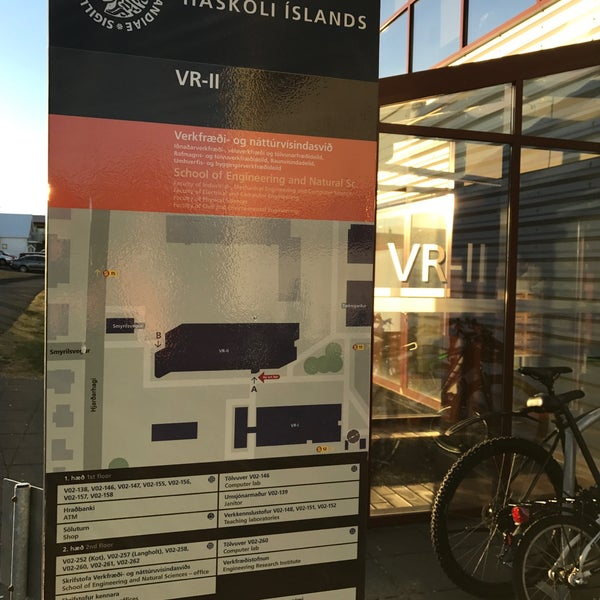
\includegraphics[height=\textwidth]{include/vr2.jpg}
        \end{column}
        \hfill
        \begin{column}{0.4\textwidth}         
            \begin{exampleblock}{Contact details:}            
            \begin{itemize}
                \item[\faEnvelope] helgaingim@hi.is
                \item[\faPhone] +354 525-4630
                \item[\faBuildingColumns] VR-II, University of Iceland
                \item[\faLinkedin] helgaingimundardottir
                \item[\faGithub] @tungufoss
            \end{itemize}
            \end{exampleblock}
            \end{column}
    \end{columns}    
\end{frame}

\end{document}

